\documentclass{standalone}
\usepackage{tikz}
\usetikzlibrary{patterns, positioning}
\usepackage[sfdefault]{ClearSans} %% option 'sfdefault' activates Clear Sans as the default text font
\usepackage[T1]{fontenc}

\begin{document}
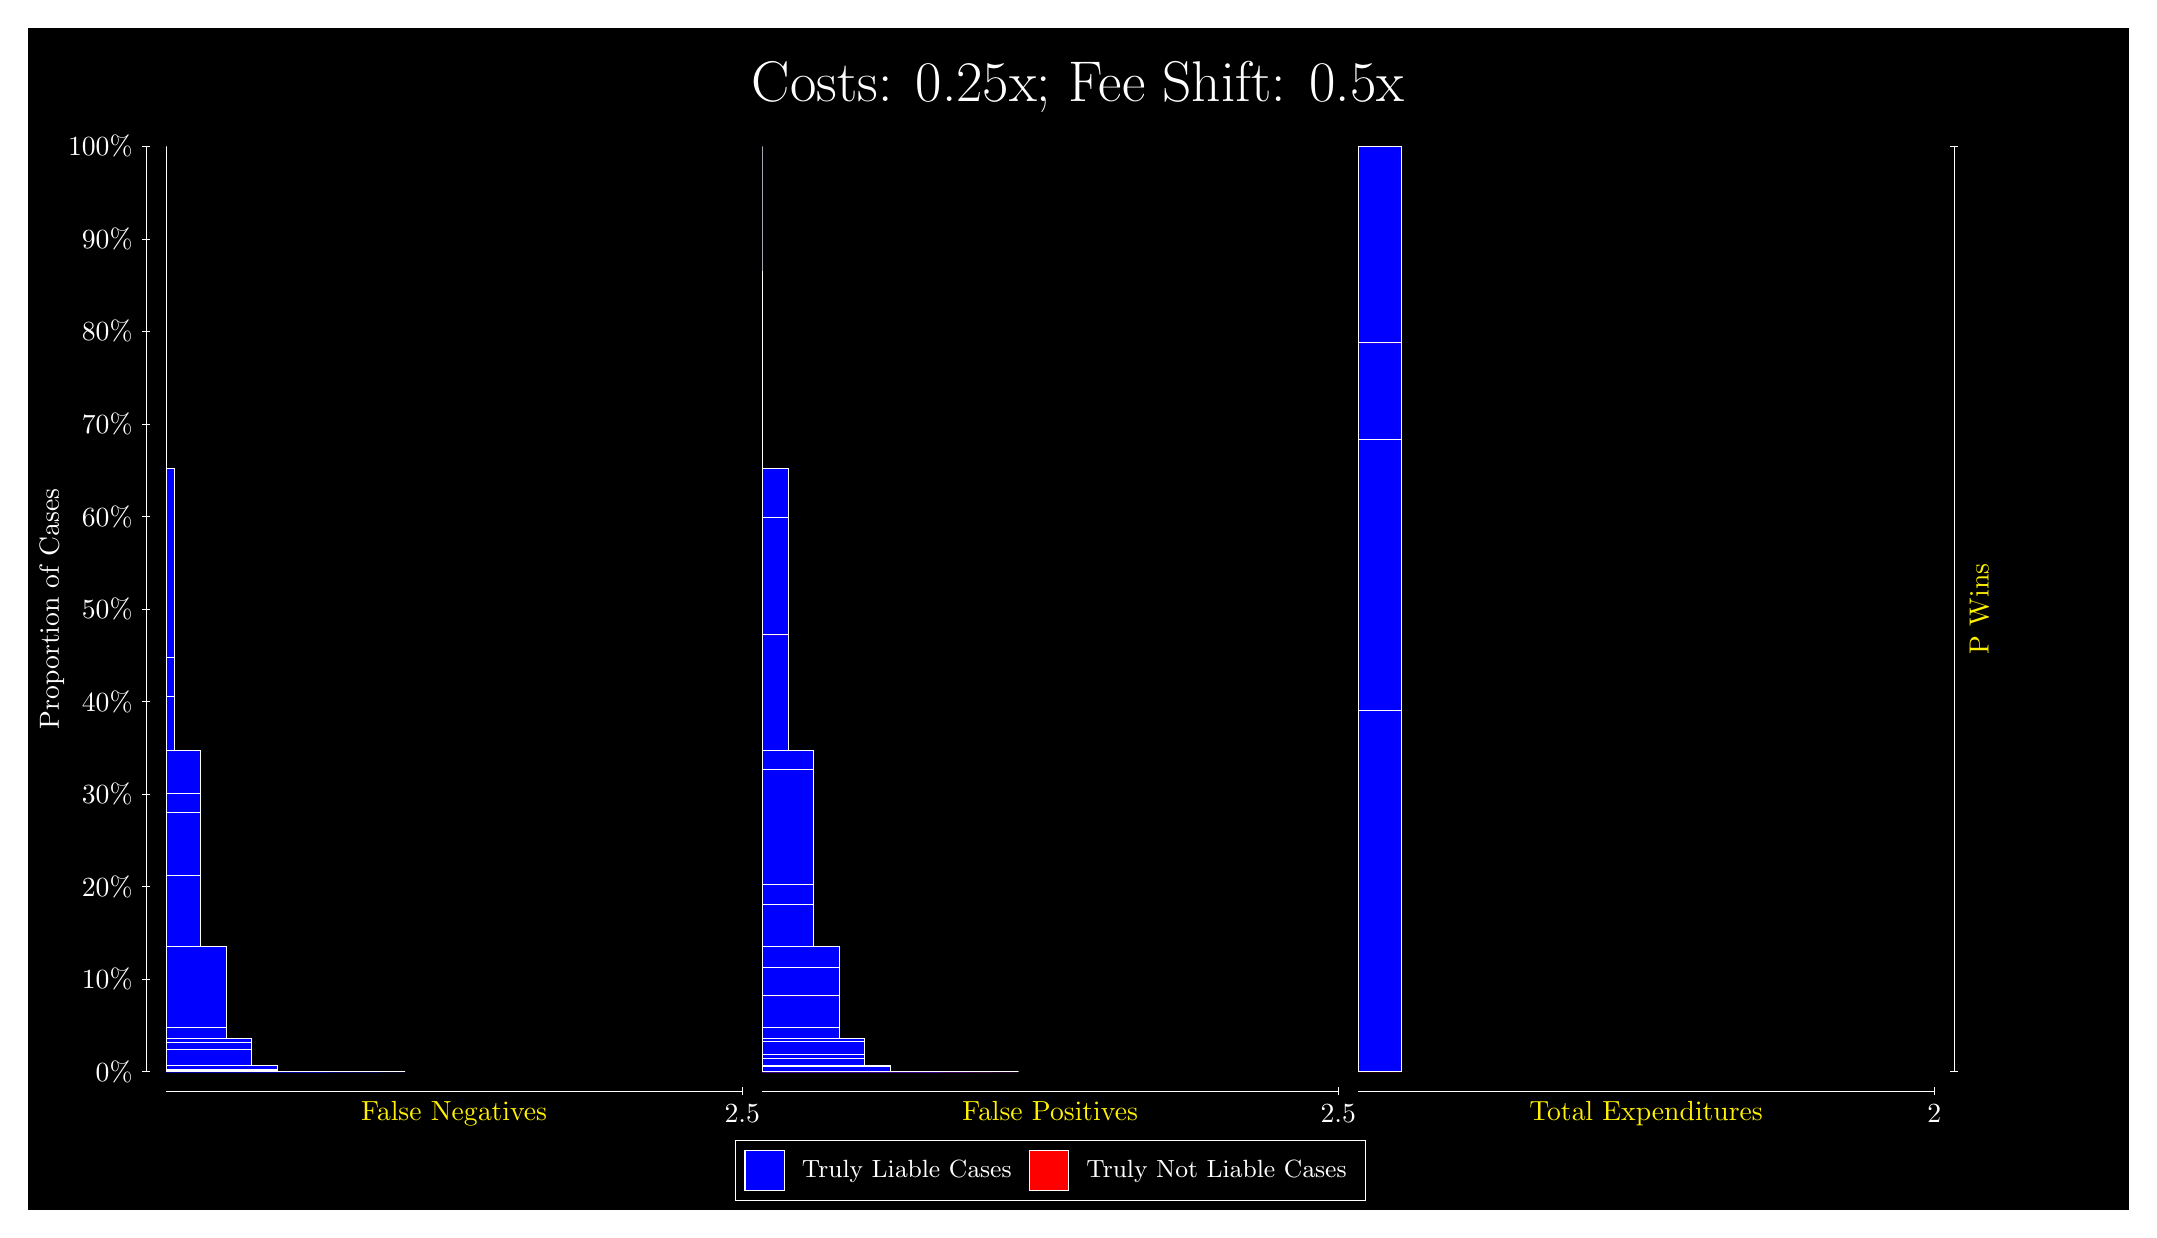
\begin{tikzpicture}
\draw[fill=black] (0,0) rectangle (26.667,15);
\draw[text=white] (0,13.5) rectangle (26.667,15) node[midway] {\huge Costs: 0.25x; Fee Shift: 0.5x};
\draw[white, very thin] (1.5,1.75) -- (1.5,13.5);
\node[rotate=90, text=white, anchor=center] at (0.3, 7.625) {Proportion of Cases};
\draw[white, very thin] (1.45,1.75) -- (1.55,1.75);
\node[text=white, anchor=east] at (1.45, 1.75) {0\%};
\draw[white, very thin] (1.45,2.925) -- (1.55,2.925);
\node[text=white, anchor=east] at (1.45, 2.925) {10\%};
\draw[white, very thin] (1.45,4.1) -- (1.55,4.1);
\node[text=white, anchor=east] at (1.45, 4.1) {20\%};
\draw[white, very thin] (1.45,5.275) -- (1.55,5.275);
\node[text=white, anchor=east] at (1.45, 5.275) {30\%};
\draw[white, very thin] (1.45,6.45) -- (1.55,6.45);
\node[text=white, anchor=east] at (1.45, 6.45) {40\%};
\draw[white, very thin] (1.45,7.625) -- (1.55,7.625);
\node[text=white, anchor=east] at (1.45, 7.625) {50\%};
\draw[white, very thin] (1.45,8.8) -- (1.55,8.8);
\node[text=white, anchor=east] at (1.45, 8.8) {60\%};
\draw[white, very thin] (1.45,9.975) -- (1.55,9.975);
\node[text=white, anchor=east] at (1.45, 9.975) {70\%};
\draw[white, very thin] (1.45,11.15) -- (1.55,11.15);
\node[text=white, anchor=east] at (1.45, 11.15) {80\%};
\draw[white, very thin] (1.45,12.325) -- (1.55,12.325);
\node[text=white, anchor=east] at (1.45, 12.325) {90\%};
\draw[white, very thin] (1.45,13.5) -- (1.55,13.5);
\node[text=white, anchor=east] at (1.45, 13.5) {100\%};

\draw[white, very thin] (24.457,1.75) -- (24.457,13.5);
\draw[white, very thin] (24.407,1.75) -- (24.507,1.75);
\node[anchor=west] at (24.407, 1.75) {};
\draw[white, very thin] (24.407,13.5) -- (24.507,13.5);
\node[anchor=west] at (24.407, 13.5) {};

\draw[white, very thin, fill=blue] (1.75,1.75) rectangle (4.7873,1.75);
\draw[white, very thin, fill=blue] (1.75,1.75) rectangle (4.462,1.75);
\draw[white, very thin, fill=blue] (1.75,1.75) rectangle (4.462,1.75);
\draw[white, very thin, fill=blue] (1.75,1.75) rectangle (4.1368,1.75);
\draw[white, very thin, fill=blue] (1.75,1.75) rectangle (3.8115,1.7502);
\draw[white, very thin, fill=blue] (1.75,1.7502) rectangle (3.8115,1.7507);
\draw[white, very thin, fill=blue] (1.75,1.7507) rectangle (3.4862,1.7574);
\draw[white, very thin, fill=blue] (1.75,1.7574) rectangle (3.4862,1.7591);
\draw[white, very thin, fill=blue] (1.75,1.7591) rectangle (3.1609,1.7691);
\draw[white, very thin, fill=blue] (1.75,1.7691) rectangle (3.1609,1.7795);
\draw[white, very thin, fill=blue] (1.75,1.7795) rectangle (3.1609,1.8271);
\draw[white, very thin, fill=blue] (1.75,1.8271) rectangle (2.8356,2.0341);
\draw[white, very thin, fill=blue] (1.75,2.0341) rectangle (2.8356,2.1242);
\draw[white, very thin, fill=blue] (1.75,2.1242) rectangle (2.8356,2.1773);
\draw[white, very thin, fill=blue] (1.75,2.1773) rectangle (2.5103,2.3077);
\draw[white, very thin, fill=blue] (1.75,2.3077) rectangle (2.5103,3.3363);
\draw[white, very thin, fill=blue] (1.75,3.3363) rectangle (2.1851,4.2373);
\draw[white, very thin, fill=blue] (1.75,4.2373) rectangle (2.1851,5.0419);
\draw[white, very thin, fill=blue] (1.75,5.0419) rectangle (2.1851,5.2899);
\draw[white, very thin, fill=blue] (1.75,5.2899) rectangle (2.1851,5.8344);
\draw[white, very thin, fill=blue] (1.75,5.8344) rectangle (1.8598,6.5213);
\draw[white, very thin, fill=blue] (1.75,6.5213) rectangle (1.8598,7.0079);
\draw[white, very thin, fill=blue] (1.75,7.0079) rectangle (1.8598,9.4156);
\draw[white, very thin, fill=red] (1.75,9.4156) rectangle (1.75,9.4156);
\draw[white, very thin, fill=blue] (1.75,9.4156) rectangle (1.75,13.5);
\draw[white, very thin, fill=red] (9.3189,1.75) rectangle (12.576,1.75);
\draw[white, very thin, fill=blue] (9.3189,1.75) rectangle (12.576,1.75);
\draw[white, very thin, fill=red] (9.3189,1.75) rectangle (12.25,1.75);
\draw[white, very thin, fill=blue] (9.3189,1.75) rectangle (12.25,1.75);
\draw[white, very thin, fill=blue] (9.3189,1.75) rectangle (11.925,1.75);
\draw[white, very thin, fill=red] (9.3189,1.75) rectangle (11.925,1.75);
\draw[white, very thin, fill=blue] (9.3189,1.75) rectangle (11.925,1.75);
\draw[white, very thin, fill=blue] (9.3189,1.75) rectangle (11.6,1.7502);
\draw[white, very thin, fill=blue] (9.3189,1.7502) rectangle (11.6,1.7503);
\draw[white, very thin, fill=red] (9.3189,1.7503) rectangle (11.6,1.7503);
\draw[white, very thin, fill=blue] (9.3189,1.7503) rectangle (11.6,1.7507);
\draw[white, very thin, fill=red] (9.3189,1.7507) rectangle (11.275,1.7507);
\draw[white, very thin, fill=blue] (9.3189,1.7507) rectangle (11.275,1.7559);
\draw[white, very thin, fill=blue] (9.3189,1.7559) rectangle (11.275,1.7574);
\draw[white, very thin, fill=blue] (9.3189,1.7574) rectangle (11.275,1.7591);
\draw[white, very thin, fill=red] (9.3189,1.7591) rectangle (10.949,1.7591);
\draw[white, very thin, fill=blue] (9.3189,1.7591) rectangle (10.949,1.8167);
\draw[white, very thin, fill=blue] (9.3189,1.8167) rectangle (10.949,1.8271);
\draw[white, very thin, fill=blue] (9.3189,1.8271) rectangle (10.624,1.919);
\draw[white, very thin, fill=blue] (9.3189,1.919) rectangle (10.624,1.9721);
\draw[white, very thin, fill=red] (9.3189,1.9721) rectangle (10.624,1.9721);
\draw[white, very thin, fill=blue] (9.3189,1.9721) rectangle (10.624,2.1322);
\draw[white, very thin, fill=blue] (9.3189,2.1322) rectangle (10.624,2.1773);
\draw[white, very thin, fill=blue] (9.3189,2.1773) rectangle (10.299,2.3088);
\draw[white, very thin, fill=blue] (9.3189,2.3088) rectangle (10.299,2.714);
\draw[white, very thin, fill=red] (9.3189,2.714) rectangle (10.299,2.714);
\draw[white, very thin, fill=blue] (9.3189,2.714) rectangle (10.299,3.0754);
\draw[white, very thin, fill=blue] (9.3189,3.0754) rectangle (10.299,3.3363);
\draw[white, very thin, fill=blue] (9.3189,3.3363) rectangle (9.9735,3.8787);
\draw[white, very thin, fill=blue] (9.3189,3.8787) rectangle (9.9735,4.1289);
\draw[white, very thin, fill=red] (9.3189,4.1289) rectangle (9.9735,4.1289);
\draw[white, very thin, fill=blue] (9.3189,4.1289) rectangle (9.9735,5.5864);
\draw[white, very thin, fill=blue] (9.3189,5.5864) rectangle (9.9735,5.8344);
\draw[white, very thin, fill=blue] (9.3189,5.8344) rectangle (9.6482,7.3002);
\draw[white, very thin, fill=red] (9.3189,7.3002) rectangle (9.6482,7.3002);
\draw[white, very thin, fill=blue] (9.3189,7.3002) rectangle (9.6482,8.7835);
\draw[white, very thin, fill=blue] (9.3189,8.7835) rectangle (9.6482,9.4156);
\draw[white, very thin, fill=blue] (9.3189,9.4156) rectangle (9.3229,9.6657);
\draw[white, very thin, fill=blue] (9.3189,9.6657) rectangle (9.3229,11.654);
\draw[white, very thin, fill=blue] (9.3189,11.654) rectangle (9.3229,11.914);
\draw[white, very thin, fill=blue] (9.3189,11.914) rectangle (9.3189,13.5);
\draw[white, very thin, fill=red] (16.888,1.75) rectangle (17.437,1.75);
\draw[white, very thin, fill=blue] (16.888,1.75) rectangle (17.437,6.3369);
\draw[white, very thin, fill=red] (16.888,6.3369) rectangle (17.437,6.3369);
\draw[white, very thin, fill=blue] (16.888,6.3369) rectangle (17.437,9.7768);
\draw[white, very thin, fill=red] (16.888,9.7768) rectangle (17.437,9.7768);
\draw[white, very thin, fill=blue] (16.888,9.7768) rectangle (17.437,11.008);
\draw[white, very thin, fill=red] (16.888,11.008) rectangle (17.437,11.008);
\draw[white, very thin, fill=blue] (16.888,11.008) rectangle (17.437,13.5);
\draw[white, very thin] (1.75,1.5) -- (9.0689,1.5);
\node[text=yellow, anchor=north] at (5.4094, 1.5) {False Negatives};
\draw[white, very thin] (9.0689,1.45) -- (9.0689,1.55);
\node[text=white, anchor=north] at (9.0689, 1.45) {2.5};

\draw[white, very thin] (9.3189,1.5) -- (16.638,1.5);
\node[text=yellow, anchor=north] at (12.978, 1.5) {False Positives};
\draw[white, very thin] (16.638,1.45) -- (16.638,1.55);
\node[text=white, anchor=north] at (16.638, 1.45) {2.5};

\draw[white, very thin] (16.888,1.5) -- (24.207,1.5);
\node[text=yellow, anchor=north] at (20.547, 1.5) {Total Expenditures};
\draw[white, very thin] (24.207,1.45) -- (24.207,1.55);
\node[text=white, anchor=north] at (24.207, 1.45) {2};

\node[text=yellow, centered, rotate=90] at (24.777, 7.625) {P Wins};

\draw (12.978300999999998,1.5) node[draw=none] (baseCoordinate) {};
\begin{scope}[align=center]
        \matrix[scale=0.5, draw=white, below=0.5cm of baseCoordinate, nodes={draw}, column sep=0.1cm]{
            \node[rectangle, draw, minimum width=0.5cm, minimum height=0.5cm, fill=blue] {}; &
            \node[draw=none, font=\small, text=white] (B) {Truly Liable Cases}; &
            \node[rectangle, draw, minimum width=0.5cm, minimum height=0.5cm, fill=red] {}; &
            \node[draw=none, font=\small, text=white] (B) {Truly Not Liable Cases}; \\
            };
\end{scope}

\end{tikzpicture}
\end{document}